\chapter{Neural Networks}\label{ch:neural-networks}
The history of neural networks can be traced back to the inception of the perceptron in 1957 by Frank Rosenblatt, a psychologist and computer scientist~\cite{rosenblatt1958perceptron}. The perceptron was a foundational model inspired by the functioning of neurons in the human brain, providing a mathematical model that enabled machines to learn from data and make predictions. It was conceptualized as a binary linear classifier, taking a set of input signals and generating an output based on the combined weighted inputs. However, the perceptron was constrained by its limitations; it could only solve linear problems.
\par The resurgence of neural networks started in the 1980s when the backpropagation algorithm was popularized (see Section~\ref{sec:backprop}). This algorithm, combined with the use of gradient descent~(\ref{subsec:gradient-descent}), allows the adjustment of weights in a multi-layer perceptron to minimize the prediction error~\cite{rumelhart1986learning}. This significant leap forward led to the development of deep learning, in which neural networks with many layers could be trained, leading to more sophisticated and accurate models.
\par The 2000s brought a further rise in the use of neural networks, primarily due to advances in hardware, particularly the use of Graphics Processing Units (GPUs) for training, and the availability of big data~\cite{schmidhuber2015deep}. As a result, neural networks, specifically deep learning, have become the cornerstone of modern artificial intelligence applications, from computer vision to natural language processing. There exist different kind of neural networks, such as convolutional neural networks~\cite{lecun1995convolutional}, popular for computer vision. In this section we focus on Fully Connected Feed-Forward Neural Networks. 
\section{Description}
A basic feed-forward neural network (FFNN), also known as a multi-layer perceptron, consists of three main components: an input layer, hidden layers, and an output layer. Each layer comprises nodes (or neurons), and each node in a layer is connected to every node in the subsequent layer through connections called weights.

The data initially enters the network through the input layer. This data then propagates forward through the hidden layers. The intermediate layers are called hidden layers because their outputs are not directly observed. In each hidden layer, the nodes receive inputs from the preceding layer, apply a weighted sum to these inputs, add a bias, and then pass the result through an activation function. The role of the activation function is to introduce non-linearity into the network, allowing it to learn and represent more complex relationships in the data.

This process continues until the output layer is reached. The output layer generates the final output of the network, which is then used for making predictions. The goal of training a neural network is to adjust the weights and biases to minimize the difference between the network's predictions and the actual values, a process typically accomplished through backpropagation and gradient descent, which we introduce in the following sections.



\subsubsection{Mathematical Details}
Before describing formally a neural network, let us first focus on the mathematical description of a single neuron, also called Linear Threshold Unit (LTU). As illustrated on Figure~\ref{fig:perceptron}, an LTU with $n$ inputs $(x_1, \dots, x_n)$ computes a weighted sum of its inputs:

\begin{equation}
    \label{eq:post-synaptic-pot}
    z = \sum_{i=1}^{n} w_i x_i + b
\end{equation}
where $(w_1, \dots, w_n)$ are the weights and $b$ is the bias term. The LTU then applies a step function to this sum:
\begin{equation}
    \label{eq:perceptron-io}
    o = 
    \begin{cases}
    1 \text{  if } z \geq 0 \\
    0 \text{  if}  z < 0
    \end{cases}
\end{equation}where $o$ is the output of the LTU.

% We note that we can rewrite $z$ as:

%\begin{equation}
%    \label{eq:post-synaptic-pot-vect}
%    z = \Vec{w}^T\cdot \Vec{x} + b\text{ , }
%\end{equation}

%where $\Vec{x} = (x_1, \dots, x_n)$ and similarly $\Vec{w} = (w_1, \dots, w_n)$ are vectors. 


\begin{figure}[ht]
    \centering
    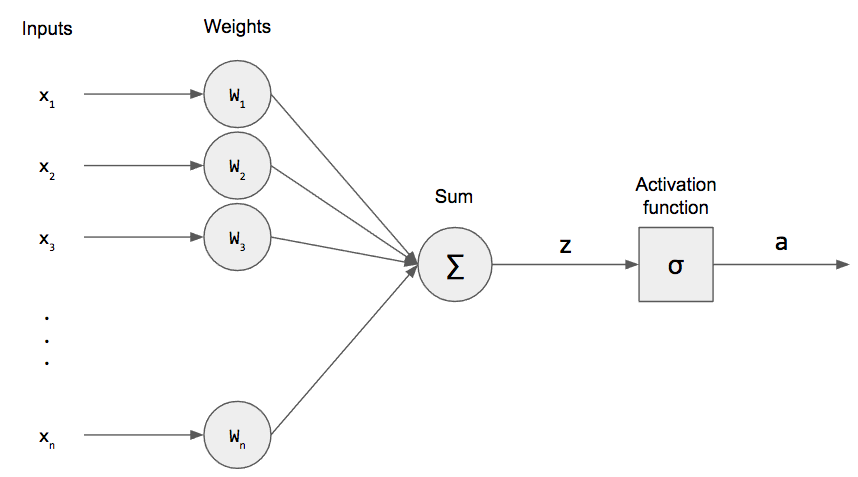
\includegraphics[width=\textwidth]{imgs/Single-Perceptron.png}
    \caption{Illustration of an LTU. The neurons are the building blocks of neural networks. 
    \\ Source: \url{https://gamedevacademy.org/perceptrons-the-first-neural-networks/}}
    \label{fig:perceptron}
\end{figure}

\par Now familiar with the mathematical expression of a perceptron, we slightly modify this latter to adapt it to the representation of a hidden layer of a neural network. Indeed, in the case of neural networks, the choice of the activation function is not limited to the step function. For the remainder of this chapter we therefore use the symbol $\sigma$ to denote any arbitrary activation function. We now consider a layer of $n$ LTUs followed by another one composed of $m$ LTUs. We write the output of the first layer in vector form:

\begin{equation}
\label{eq:output-vector}
\Vec{a}^{(1)} =
\begin{bmatrix}
o_1 \\
o_2 \\
\vdots \\
o_n
\end{bmatrix}
\end{equation}
If $\Vec{Z}^{(2)}$ is the output vector of the second layer before applying the activation function, where each entry of the vector $\Vec{Z}^{(2)}$ corresponds to an LTU, $\Vec{Z}^{(2)}$ can be expressed as follows:
\begin{equation}
\label{eq:ouput-layer}
 \Vec{Z}^{(2)} =
\begin{bmatrix}
z_1^{(2)} \\
z_2^{(2)} \\
\vdots \\
z_m^{(2)}
\end{bmatrix}
=
\begin{bmatrix}
o_1w_{11} + o_2w_{12} + \dots +o_i w_{1i} + b_1\\
o_1w_{21} + o_2w_{22} + \dots +o_i w_{2i} + b_2\\
\vdots \\
o_1w_{m1} + o_2w_{m2} + \dots +o_i w_{mi} + b_m
\end{bmatrix}
\end{equation}
where we have used Equation~\eqref{eq:post-synaptic-pot}. Indeed, for the $k^{\text{th}}$ LTU among the $m$ LTUs of the second layer, Equation~\eqref{eq:post-synaptic-pot} can be written as

\begin{equation*}
z_k = \sum_{i=1}^{m} x_i w_{ki} + b_k \text{ .}
\end{equation*}

The vector $\Vec{Z}^{(2)}$ can be rewritten as a dot product between the weight matrix $\mathbf{W}^{(2)}$ of layer 2 and the output vector $\Vec{a}^{(1)}$ given by Equation~\eqref{eq:output-vector}:

\begin{equation}
\label{eq:one-layer-output-detail}
\Vec{Z}^{(2)} =
\begin{bmatrix}
    w_{11} & w_{12} & \dots & w_{1n} \\
    w_{21} & w_{22} & \dots & w_{2n} \\
    \vdots & \vdots & \ddots & \vdots \\
    w_{m1} & w_{m2} & \dots & w_{jn}
\end{bmatrix}
\begin{bmatrix}
    o_1 \\
    o_2 \\
    \vdots \\
    o_n
\end{bmatrix}
+
\begin{bmatrix}
    b_1 \\
    b_2 \\
    \vdots \\
    b_m
\end{bmatrix}
\end{equation}
or equivalently

\begin{equation}
    \label{eq:output-layer-matrix}
    \Vec{Z}^{(2)} = \mathbf{W}^{(2)}\cdot \Vec{a}^{(1)} + \Vec{b}^{(2)}
\end{equation}

Finally, we can express the outputs of layer 2 in terms of the weights and biases of this layer and, the outputs of the previous one. For any layer $l$, and the preceding layer $l-1$, this can be written as:

\begin{equation}
\label{eq:output-any-layer}
\Vec{a}^{(l)} = \sigma^{(l)}\left(\Vec{Z}^{(l)}\right) = \sigma^{(l)}\left(\mathbf{W}^{(l)} \cdot \Vec{a}^{(l-1)} + \Vec{b}^{(l)}\right)
\end{equation}
where the activation function $\sigma$ is applied to each element of the vector $\Vec{Z_l}$.

A neural network is a mathematical function that can be represented as a graph of interconnected neurons (see Figure~\ref{fig:mlp}). Mathematically, this function can be described as a series of nested non-linear functions. The output of each function feeds into the input of the next function, and so on, until the final output of the network is produced. Formally, this is expressed as:

\begin{align}
f &\text{: } \mathbb{R}^n \to \mathbb{R}^m\nonumber\\
f &= g \circ f_L \circ f_{L-1} \dots f_2 \circ f_1 (x) \text{ with, }
\end{align}

\begin{align}
f_l &\text{: } \mathbb{R}^{n_l} \to \mathbb{R}^{n_{l-1}}\nonumber\\
f_l(x) &= \sigma^{(l)}(\mathbf{W}^{(l)} \cdot \Vec{x} + b^{(l)})
\end{align}

where $n$ is the dimension of the input $\Vec{x}$, $m$ is the dimension of the output $\Vec{y}$, $g$ is the \emph{output function}, and each $f_l$ is itself a composed multivariate function. In terms of what we have described with Equations~\eqref{eq:output-layer-matrix} and~\eqref{eq:output-any-layer}, this can be written in a more intuitive form as follows:

\begin{figure}[ht]
\centering
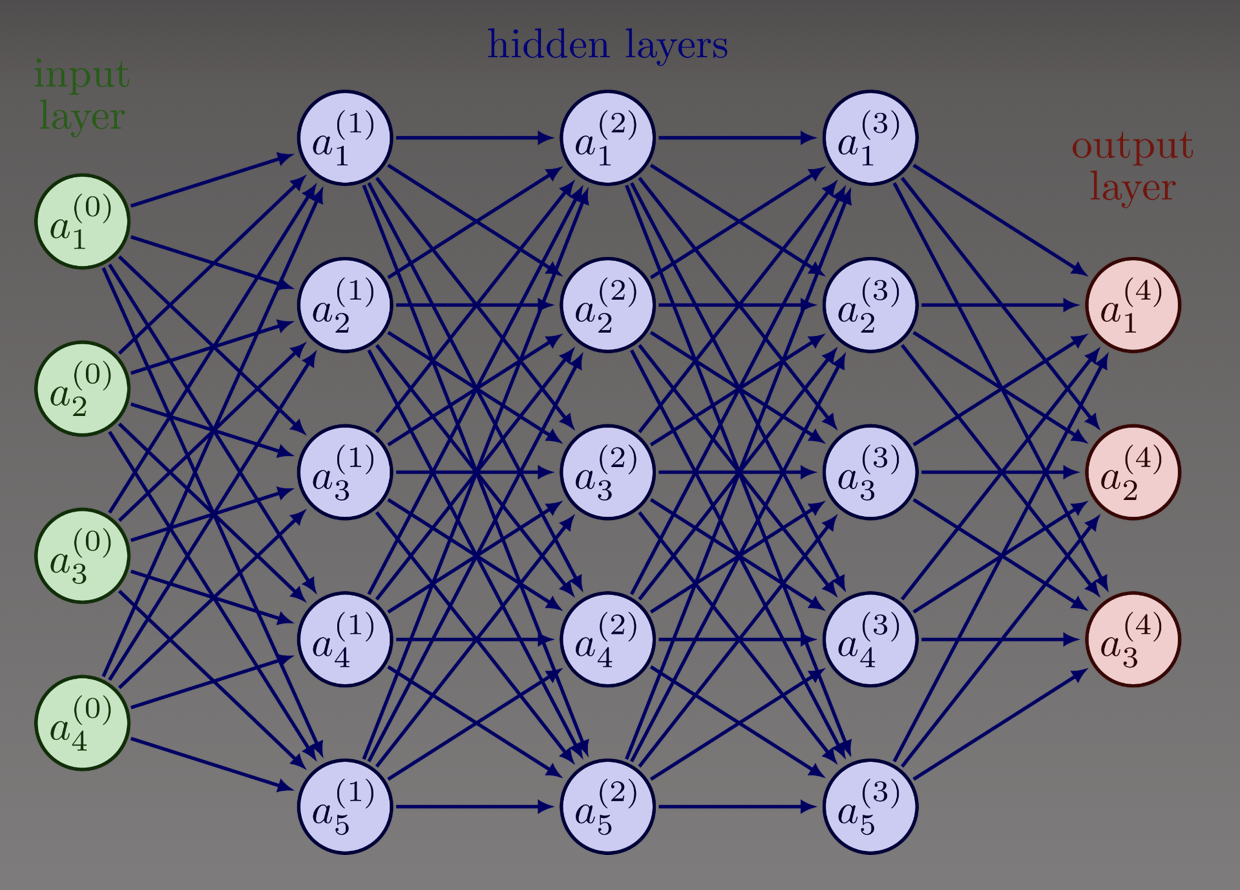
\includegraphics[width=\textwidth]{imgs/Architecture-perceptron-multi-couches-2.png}
\caption{Structure of a neural network with three hidden layers.}
\label{fig:mlp}
\end{figure}

\begin{equation}
\label{eq:mlp}
\hat{f}(\mathbf{x}) = g\left( \mathbf{W}^{(L-1)} \sigma^{(L-2)} \left( \cdots \sigma^{(2)} \left(
\mathbf{W}^{(2)} \sigma^{(1)} \left( \mathbf{W}^{(1)} \mathbf{x} + b^{(1)} \right) + b^{(2)} \right) \cdots \right) +
b^{(L-1)} \right)
\end{equation}
where $\hat{f}(\mathbf{x})$ denotes here the predicted output for a neural networks with $L$ layers. In other words, each hidden layer is calculated by applying a linear transformation $\mathbf{W}^{(l)} \cdot$ to the output of the previous layer, followed by a non-linear activation function $\sigma^{(l)}(\cdot)$. The final output is calculated by applying an output function $g$ to the output of the last hidden layer. The form of $g$ depends on the problem we aim to solve. In the case we are interested in, regression, $g$ is a simple linear function:

\begin{equation}
\label{eq:output-function}
g(\Vec{x}) = \mathbf{W}^{(L)} \cdot \Vec{x} + \Vec{b}^{(L)}
\end{equation}


We have formally described a forward pass of a Feed-forward Neural Network for input data $\Vec{x}$, given weights $w$ and biases $b$. These latter elements, which we will denote as $\theta$, can be initialized in various ways. We do not wish to delve into these details here and we just consider random initialization. Once initialized, we aim to adjust these weights and biases so that the function $\hat{f}(\Vec{x})$, approximated by the network, closely mirrors the true value of $f(\Vec{x})$. To this end, we require a method to tweak these parameters.

\subsection{Loss Function}

First, we quantify the error produced by the network using a \emph{loss function}, generally defined as follows:

\begin{equation}
\label{eq:def-loss-function}
\mathcal{L}(\theta) = \frac{1}{2n} \sum_{i=1}^n \left[\hat{y}_{\theta}^{(i)} - y^{(i)}\right]^2
\end{equation}
Here, $\theta$ represents the set of parameters, $\hat{y} = \hat{f}(\Vec{x})$ is the value predicted by the network, and $y=f(\Vec{x})$ is the actual value. We have employed the Mean Squared Error (MSE) as the loss function, commonly used for regression problems. The factor $1/2$ is added to simplify the factor of 2 that arises when calculating the gradient of $\mathcal{L}$.

\subsection{Gradient Descent}\label{subsec:gradient-descent}

We now have a function to measure the error made by the neural network. Naturally, for the network to be as efficient as possible, the error should be as low as possible. Therefore, we aim to minimize the loss function $\mathcal{L}$ from equation~\eqref{eq:def-loss-function}. The algorithm used for this process is called \emph{gradient descent}. This algorithm, proposed by Cauchy~\cite{cauchymethode} is based on the idea that if $F(\Vec{x})$ is a multivariate function defined and derivable in the vicinity of a point $\mathbf {a}$, then $ F(\mathbf {x} )$ decreases the fastest if we start from $\Vec{a}$ in the direction opposite to the gradient $\nabla F(\Vec{a})$.

In the parameter space $\theta$, we want to move towards a point $\Vec{\theta}$ that reduces the error $\mathcal{L}\left( \theta \right)$. Thus, following the gradient algorithm's principle, we want to change the point $\Vec{\theta}_{n}$'s coordinates in the direction given by $-\nabla \mathcal{L}(\Vec{\theta})$. We also need to define a unit length, or step size, by which we want to change the point's coordinates. This unit length is called the \emph{learning rate} and is often denoted as $\eta \in \mathbb{R}^+$. Finally, the change in parameters can be described as:

\begin{equation}
\label{eq:gradient-descent}
\Vec{\theta}_{n+1} = \Vec{\theta}_n - \eta \nabla \mathcal{L}(\Vec{\theta}_n)
\end{equation}

The choice of step size, $\eta$, is crucial. Using a small $\eta$ value could slow convergence and potentially trap the algorithm in a local minimum. On the other hand, choosing a large $\eta$ value could lead to divergence. The external parameters composing a neural network, and that are not trained, are called \emph{hyperparameters}. The choice of these hyperparameters is primordial and can decide whether a model is going to be successful or not.

\subsection{Gradient Descent Algorithms}
In practice, for networks containing a large number of parameters (on the order of $10^8-10^9$), iterating on each of these parameters following equation~\eqref{eq:gradient-descent} is not feasible. As a result, additional algorithms have been developed to circumvent this problem. We briefly present stochastic gradient descent, commonly used, as well as the Adam and L-BFGS algorithms, often employed in conjunction with PINNs.

\subsubsection{Stochastic Gradient Descent}
Stochastic Gradient Descent differs from ordinary gradient descent in that instead of taking into account all training examples to compute the gradient of the error, it selects just one example (or a small batch, in what's called the mini-batch method) at each iteration. Consequently, the gradient is computed and the weight updates are performed far more frequently, which can lead to faster convergence, though the individual steps are noisier. Mathematically, the iteration of a SGD step for a given weight is the same as for equation~\eqref{eq:gradient-descent}.

\subsubsection{Adaptive Moment Estimation}
The Adaptive Moment Estimation algorithm (Adam) is an optimization method introduced by Kingma and Ba~\cite{kingma2017adam}. This method is specifically designed for training deep neural networks. Its main advantage is that it adjusts the learning rate for each model weight individually, based on the estimates of the first moment (the mean) and the second moment (the uncentered variance) of the gradients.

The Adam algorithm can be detailed as follows:
\begin{enumerate}
    \item Initialize the first and second order moments as follows:
    \begin{itemize}
        \item $m_0=0$ (Initialize the 1st moment)
        \item $v_0=0$ (Initialize the 2nd moment)
    \end{itemize}
    \item For each iteration step $t$ (starting from $t=1$), compute the gradient $g_t$ of the error function with respect to the current parameters $\theta_t$.
    \item Update the moment estimates as follows:
    \begin{itemize}
        \item $m_t = \beta_1 \cdot m_{t-1} +(1-\beta_1) \cdot g_t$
        \item $v_t = \beta_2 \cdot v_{t-1} + (1-\beta_2) \cdot g_{t}^{2}$ 
        where $\beta_1$ and $\beta_2$ are hyperparameters controlling the decay of moments (typically 0.9 and 0.999 respectively).
    \end{itemize}
    \item Correct the moments for the initial bias towards zero as follows:
        \begin{itemize}
        \item $\hat{m}^t = \dfrac{m_t}{1 - \beta_{1}^{t}}$
        \item $\hat{v}^t = \dfrac{v_t}{1 - \beta_{2}^{t}}$
    \end{itemize}
    \item Lastly, update the parameters using the bias-corrected moments:

    $$\theta_{t+1} = \theta_t - \eta \cdot \dfrac{\hat{m}^t}{\sqrt{\hat{v}^t} + \epsilon}$$

where $\eta$ is the learning rate and $\epsilon$ is a small number to avoid division by zero (typically $10^{-8}$).
\end{enumerate}

The computation of first and second order moments enables Adam to adjust the learning rate of each parameter individually, which can help speed up the convergence of training, particularly in deep neural networks with many parameters.


\subsubsection{Limited-memory BFGS}
The BFGS (Broyden–Fletcher–Goldfarb–Shanno) algorithm is a quasi-Newtonian method that uses a formula to update the approximation of the  Hessian matrix (or its inverse) at each iteration. As an example, from an initial value $\Vec{x}_0$ and an approximated Hessian matrix $B_0$, the following iterations are repeated until $\Vec{x}$ converges towards the solution:
\begin{enumerate}
    \item Find the direction of descent $\Vec{p}_k$ by solving $B_k\Vec{p}_k = - \nabla f(\Vec{x}_k)$
    \item Perform a linear search to find the optimal step size $\alpha_k$, in the direction found in step 1, and then udpate
        $\Vec{x}_{k+1} = \Vec{x}_k + \alpha_k \Vec{p}_k = \Vec{x}_k + \Vec{s}_k$
    \item $\Vec{y}_k = f(\Vec{x}_{k+1}) - f(\Vec{x}_k)$
    \item $B_{k+1} = B_k + \left(\Vec{y}_k \Vec{y}_k^T\right)/\left(\Vec{y}_k^T \Vec{s}_k \right) - \left( B_k \Vec{s}_k\Vec{s}_k^TB_k\right)/\left(\Vec{s}_k^T B_k \Vec{s}_k\right)$
\end{enumerate} where $f(\Vec{x})$ is the function to minimize. This algorithm can also be expressed using the inverse Hessian matrix $H_k \equiv B_k^{-1}$. However, for problems with a large number of variables, storing and manipulating matrices $B_k$ or $H_k$ can be very costly in terms of memory and computation time.

This is where the L-BFGS (Limited-memory BFGS) algorithm~\cite{nocedal1980updating} comes into play. It is specifically designed for problems with a large number of variables. Instead of storing the complete inverse Hessian matrix, L-BFGS only stores a few vectors representing the differences in gradients and positions from previous iterations. Using these vectors, it's possible to compute an approximation of the inverse Hessian matrix, which allows for the next iteration to be performed.

The method used to compute this approximation is called the two-loop algorithm. The first loop, going from the current iteration to the current iteration minus $m$, uses the stored information to compute an approximation of the gradient. The second loop, going from the current iteration minus $m$ to the current iteration, uses the same information to compute the search direction.

\section{Back-propagation}\label{sec:backprop}

Backpropagation is an algorithm that enables the computation of the gradient of the error, thereby permitting the adjustment of network parameters according to~\eqref{eq:gradient-descent}. Prior to describing the algorithm, we compute the gradients with respect to each network parameter.

Starting from the gradient in Equation~\eqref{eq:gradient-descent} and employing the chain rule together with equation~\eqref{eq:post-synaptic-pot}, we may express:

\begin{equation}
\label{eq:gradient-wrt-weights}
\frac{\partial \L}{\partial w_{ik}^{(l)}} = \frac{\partial \L}{\partial z_{k}^{(l)}}\frac{\partial z_{k}^{(l)}}{\partial w_{ik}^{(l)}} = \frac{\partial \L}{\partial z_{k}^{(l)}} a_{k}^{(l-1)}
\end{equation}
Similarly, it can be shown that:

\begin{equation}
\label{eq:gradient-wrt-bias}
\frac{\partial \L}{\partial b_{k}^{(l)}} = \frac{\partial \L}{\partial z_{k}^{(l)}}\frac{\partial z_{k}^{(l)}}{\partial b_{k}^{(l)}} = \frac{\partial \L}{\partial z_{k}^{(l)}}
\end{equation}

Now, to fully express equations~\eqref{eq:gradient-wrt-weights} and~\eqref{eq:gradient-wrt-bias}, it suffices to determine $\frac{\partial \L}{\partial z_{k}^{(l)}}$. We aim to express this partial derivative in terms of data originating from the output layer. Information is propagated layer by layer, from right to left. Therefore, we need to express the derivative of the error with respect to $z^{(l)}$ based on this same quantity originating from layer $l+1$. This results in:

\begin{equation}
\label{eq:gradient-wrt-z}
\frac{\partial \L}{\partial z_{k}^{(l)}} = \sum_{m} \frac{\partial \L}{\partial z_{m}^{(l+1)}}\frac{\partial z_{m}^{(l+1)}}{\partial z_{k}^{(l)}} = \sum_{m} \frac{\partial \L}{\partial z_{m}^{(l+1)}}\frac{\partial z_{m}^{(l+1)}}{\partial a_{k}^{(l)}}\frac{\partial a_{k}^{(l)}}{\partial z_{k}^{(l)}}\text{ ,}
\end{equation}
where $m$ represents a neuron in layer $l+1$. Based on equation~\eqref{eq:output-any-layer} and equation~\eqref{eq:output-layer-matrix}, it follows that:

\begin{equation*}
\frac{\partial z_{m}^{(l+1)}}{\partial a_{k}^{(l)}} = w_{km}^{(l+1)}
\end{equation*}

and

\begin{equation*}
\frac{\partial a_{k}^{(l)}}{\partial z_{k}^{(l)}} = \sigma'(z_{k}^{(l)})
\end{equation*}

As a result, \eqref{eq:gradient-wrt-z} becomes:

\begin{figure}
    \centering
    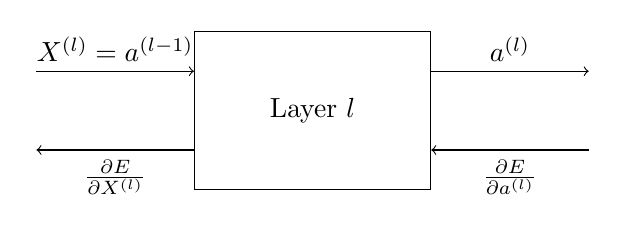
\begin{tikzpicture}

        \node[draw,rectangle,minimum height=2cm,minimum width=3cm,align=center] (layer) at (0,0) {Layer $l$};
        
        \draw[<-] ([yshift=0.5cm]layer.west) -- ++(-2,0) node[midway,above] {$X^{(l)}=a^{(l-1)}$};
        \draw[->] ([yshift=-0.5cm]layer.west) -- ++(-2,0) node[midway,below] {$\frac{\partial E}{\partial X^{(l)}}$};
        
        \draw[->] ([yshift=0.5cm]layer.east) -- ++(2,0) node[midway,above] {$a^{(l)}$};
        \draw[<-] ([yshift=-0.5cm]layer.east) -- ++(2,0) node[midway,below] {$\frac{\partial E}{\partial a^{(l)}} $};
    \end{tikzpicture}
    \caption{Hidden layer $l$ of a neural network. Layer $l$ takes as input the data $\Vec{X}^{(l)}$, the output from the previous layer $l-1$, and outputs the vector $\Vec{a}^{(l)}$, as depicted by the upper arrows. The lower arrows illustrate the derivatives of the error with respect to the inputs of the previous layer, when backpropagation is performed.}
    \label{fig:illustration-layer-l}
\end{figure}

\begin{equation}
\label{eq:gradient-wrt-z-final}
\frac{\partial \L}{\partial z_{k}^{(l)}} = \sum_{m} \frac{\partial \L}{\partial z_{m}^{(l+1)}}w_{km}^{(l+1)}\sigma'(z_{k}^{(l)}) \text{ ,}
\end{equation}
where $\sigma'$ is the derivative of the activation function for hidden layers. It is assumed here that all hidden layers have the same activation function. If this is not the case, the expression remains the same, but one must indicate the function $\sigma$'s layer affiliation. The equations~\eqref{eq:gradient-wrt-weights},~\eqref{eq:gradient-wrt-bias} and~\eqref{eq:gradient-wrt-z-final} can be rewritten in a more concise manner using vector notation:

\begin{equation}
    \label{eq:gradient-wrt-weights-matrix}
    \frac{\partial \L}{\partial \Vec{W}^{(l)}} = \frac{\partial \L}{\partial \Vec{Z}^{(l)}} \cdot \Vec{a}^{(l-1)T}
\end{equation}

\begin{equation}
    \label{eq:gradient-wrt-bias-matrix}
    \frac{\partial \L}{\partial \Vec{b}^{(l)}} = \frac{\partial \L}{\partial \Vec{Z}^{(l)}}
\end{equation}

\begin{equation}
    \label{eq:gradient-wrt-z-final-matrix}
    \frac{\partial \L}{\partial \Vec{Z}^{(l)}} = \left(\Vec{W}^{(l+1)T} \cdot \frac{\partial \L}{\partial \Vec{Z}^{(l+1)}} \right) \odot \sigma'\left(\Vec{Z}^{(l)}\right)
\end{equation}
where $\odot$ is the Hadamard product. For the output layer, it simply comes:

\begin{equation}
\label{eq:gradient-output-layer}
    \frac{\partial\L}{\partial \Vec{W}^{(L)}} = \left(\hat{\Vec{y}} - \Vec{y}\right) g'(\Vec{a}^{(L)}) \Vec{a}^{(L-1)T}
\end{equation}

\subsubsection{Algorithm}
The backpropagation algorithm can be summarized in three main steps:
\begin{enumerate}
    \item Compute the forward pass for each input-output pair and store the results $\hat{y}$, $\Vec{a}^{(l)}$, $\Vec{Z}^{(l)}$ by proceeding from layer 1, the input layer, to layer $L$, the output layer.
    \item Compute the backpropagation phase for each input-output pair and store the results $\frac{\partial \L}{\partial w_{ik}^{(l)}}$ for each weight $ w_{ik}^{(l)}$ connecting node $i$ in layer $l-1$ to a node $k$ in layer $l$, by proceeding from layer $L$, the output layer, to layer 1, the input layer. This process is illustrated in Figure~\ref{fig:illustration-layer-l} for any given layer $l$. The steps for computing the backward phase are as follows: 
    \begin{enumerate}
        \item Evaluate the error term for the final layer using equation~\eqref{eq:gradient-output-layer}.
        \item Back-propagate the error terms for the hidden layers, starting from the last hidden layer $l=L-1$, by repeatedly applying equation~\eqref{eq:gradient-wrt-z-final}.
        \item Evaluate the partial derivatives of the error with respect to $w_{ik}^{(l)}$ using equation~\eqref{eq:gradient-wrt-weights}.
    \end{enumerate}
    \item Update the parameters according to equation~\eqref{eq:gradient-descent}.
\end{enumerate}

One full cycle of this algorithm is called an \emph{epoch}.
\section{Automatic Differentiation}\label{sec:AD}

Automatic-differentiation, also known as algorithmic differentiation (AD), is a collection of techniques used for evaluating the derivatives of a numerical function with high precision. It is grounded on the fact that every numerical function, regardless of its complexity, is ultimately a composition of several elementary functions (such as addition, multiplication, exponential, logarithm, etc.) and their derivatives are well known.

Automatic differentiation employs the chain rule to decompose the derivatives of complex functions into a series of derivatives of elementary functions. The idea is to apply the chain rule at each step of the function evaluation, storing intermediate results, which allows calculating the derivatives in a single pass through the function.

There are two modes of automatic differentiation. The \textbf{Forward mode} (or direct mode) computes the derivatives of all outputs with respect to one input. Suppose we have a function $\Vec{y} = f(\Vec{x})$, where $\Vec{x}$ is a vector and $\Vec{y}$ is a vector. The forward mode calculates the derivatives $\frac{\partial y_i}{\partial x_j}$ for all $i$ and a given $j$. On the other hand, the \textbf{Reverse mode} (or backward mode) computes the derivatives of one output with respect to all inputs. The reverse mode calculates the derivatives $\frac{\partial y_i}{\partial x_j}$ for a given $i$ and all $j$.

Both modes have their uses, but in deep learning, the reverse mode is most often used because we are typically interested in the gradient of a scalar cost function with respect to all model parameters.
Auto-differentiation has several advantages over other differentiation methods, including numerical and symbolic methods, which make it particularly appealing in deep learning.

\begin{itemize}
    \item Precision: Unlike numerical differentiation (which uses finite differences to estimate derivatives), AD is exact up to floating-point error. Numerical methods can introduce significant error, either due to machine precision (if the difference interval is too small), or due to a rough approximation of the derivative (if the interval is too large).
    \item Efficiency: AD is generally more efficient than symbolic differentiation, which can generate very complex expressions when working with complex functions or high dimensions (the so-called "expression swell" problem). AD, on the other hand, calculates the derivatives using a sequence of elementary operations (addition, multiplication, etc.) and corresponding derivation rules. This allows for more efficient calculation of derivatives and at a lower computational cost.
    \item Gradient calculation for multivariate functions: AD is particularly useful for calculating the gradient (or the Jacobian, or the Hessian) of multivariate functions. This is very relevant for deep learning, where we work with loss functions depending on thousands, or even millions of parameters.
\end{itemize}

Popular deep learning frameworks, such as PyTorch~\cite{NEURIPS2019_9015} that we use for this work, take advantage of automatic differentiation for fast computation. In fact, as mentioned in the introduction, one could argue that the use of PINNs, and their efficiency for quickly solving PDEs, relies strongly on this property of neural networks. 

\section{The Universal Approximation Theorem}\label{sec:univ-approx}
The universal approximation theorem asserts that a neural network with a single hidden layer can approximate any continuous function on compact subsets of $\mathbb{R}^n$, provided that the hidden layer's activation function is non-constant, bounded, and continuous.

The theorem is generally attributed to Cybenko~\cite{cybenko1989} for the case of sigmoid activation neural networks, and was extended by Hornik~\cite{hornik1991approximation} to cover the case of other activation functions.

To formalize it mathematically, let's suppose that $\phi : \mathbb{R} \rightarrow \mathbb{R}$ is a non-constant, bounded, and continuous activation function. For a continuous function $f : \mathbb{R}^n \rightarrow \mathbb{R}$ defined on a compact $K$ of $\mathbb{R}^n$, for any $\epsilon > 0$, there exists a natural number L and weight vectors $\Vec{w}^{(1)}, \dots, \Vec{w}^{(L)} \in \mathbb{R}^n$, scalars $b_1, \dots, b_L$ and $v \in \mathbb{R}$ such that:

\begin{equation}
| f(x) - F(x; v, w, b) | < \epsilon
\end{equation}
for every $x$ in $K$, where

\begin{equation}
F(x; v, w, b) = \sum_{k=1}^{L} v_k \phi(w_{k} x + b_k)
\end{equation}
Here, $F(x; v, w, b)$ represents the output of a one hidden layer neural network with $L$ neurons and an activation function $\phi$.

This means it's possible to construct a neural network that can approximate the function $f$ as closely as we desire, by appropriately choosing weights and biases. We assume this result to hold, as it motivates the use of neural networks for approximating potentials from Chapter~\ref{ch:galaxies-theory}, but the interested reader can find a formal proof in Appendix~\ref{app:approx-theorem}.